\documentclass{article}
\usepackage[paperwidth=182mm,paperheight=257mm,margin=0mm]{geometry}
\usepackage{fontspec,xcolor,tikz}\usetikzlibrary{calc}
\setmainfont{Noto Serif CJK KR}\setsansfont{Noto Sans CJK KR}
\definecolor{navy}{HTML}{14283F}\definecolor{gold}{HTML}{C9A24B}\definecolor{paper}{HTML}{F4EFE3}
\pagestyle{empty}\setlength{\parindent}{0pt}
\begin{document}
% 앞표지
\begin{tikzpicture}[remember picture,overlay]
\node[anchor=south west,inner sep=0] at (current page.south west) {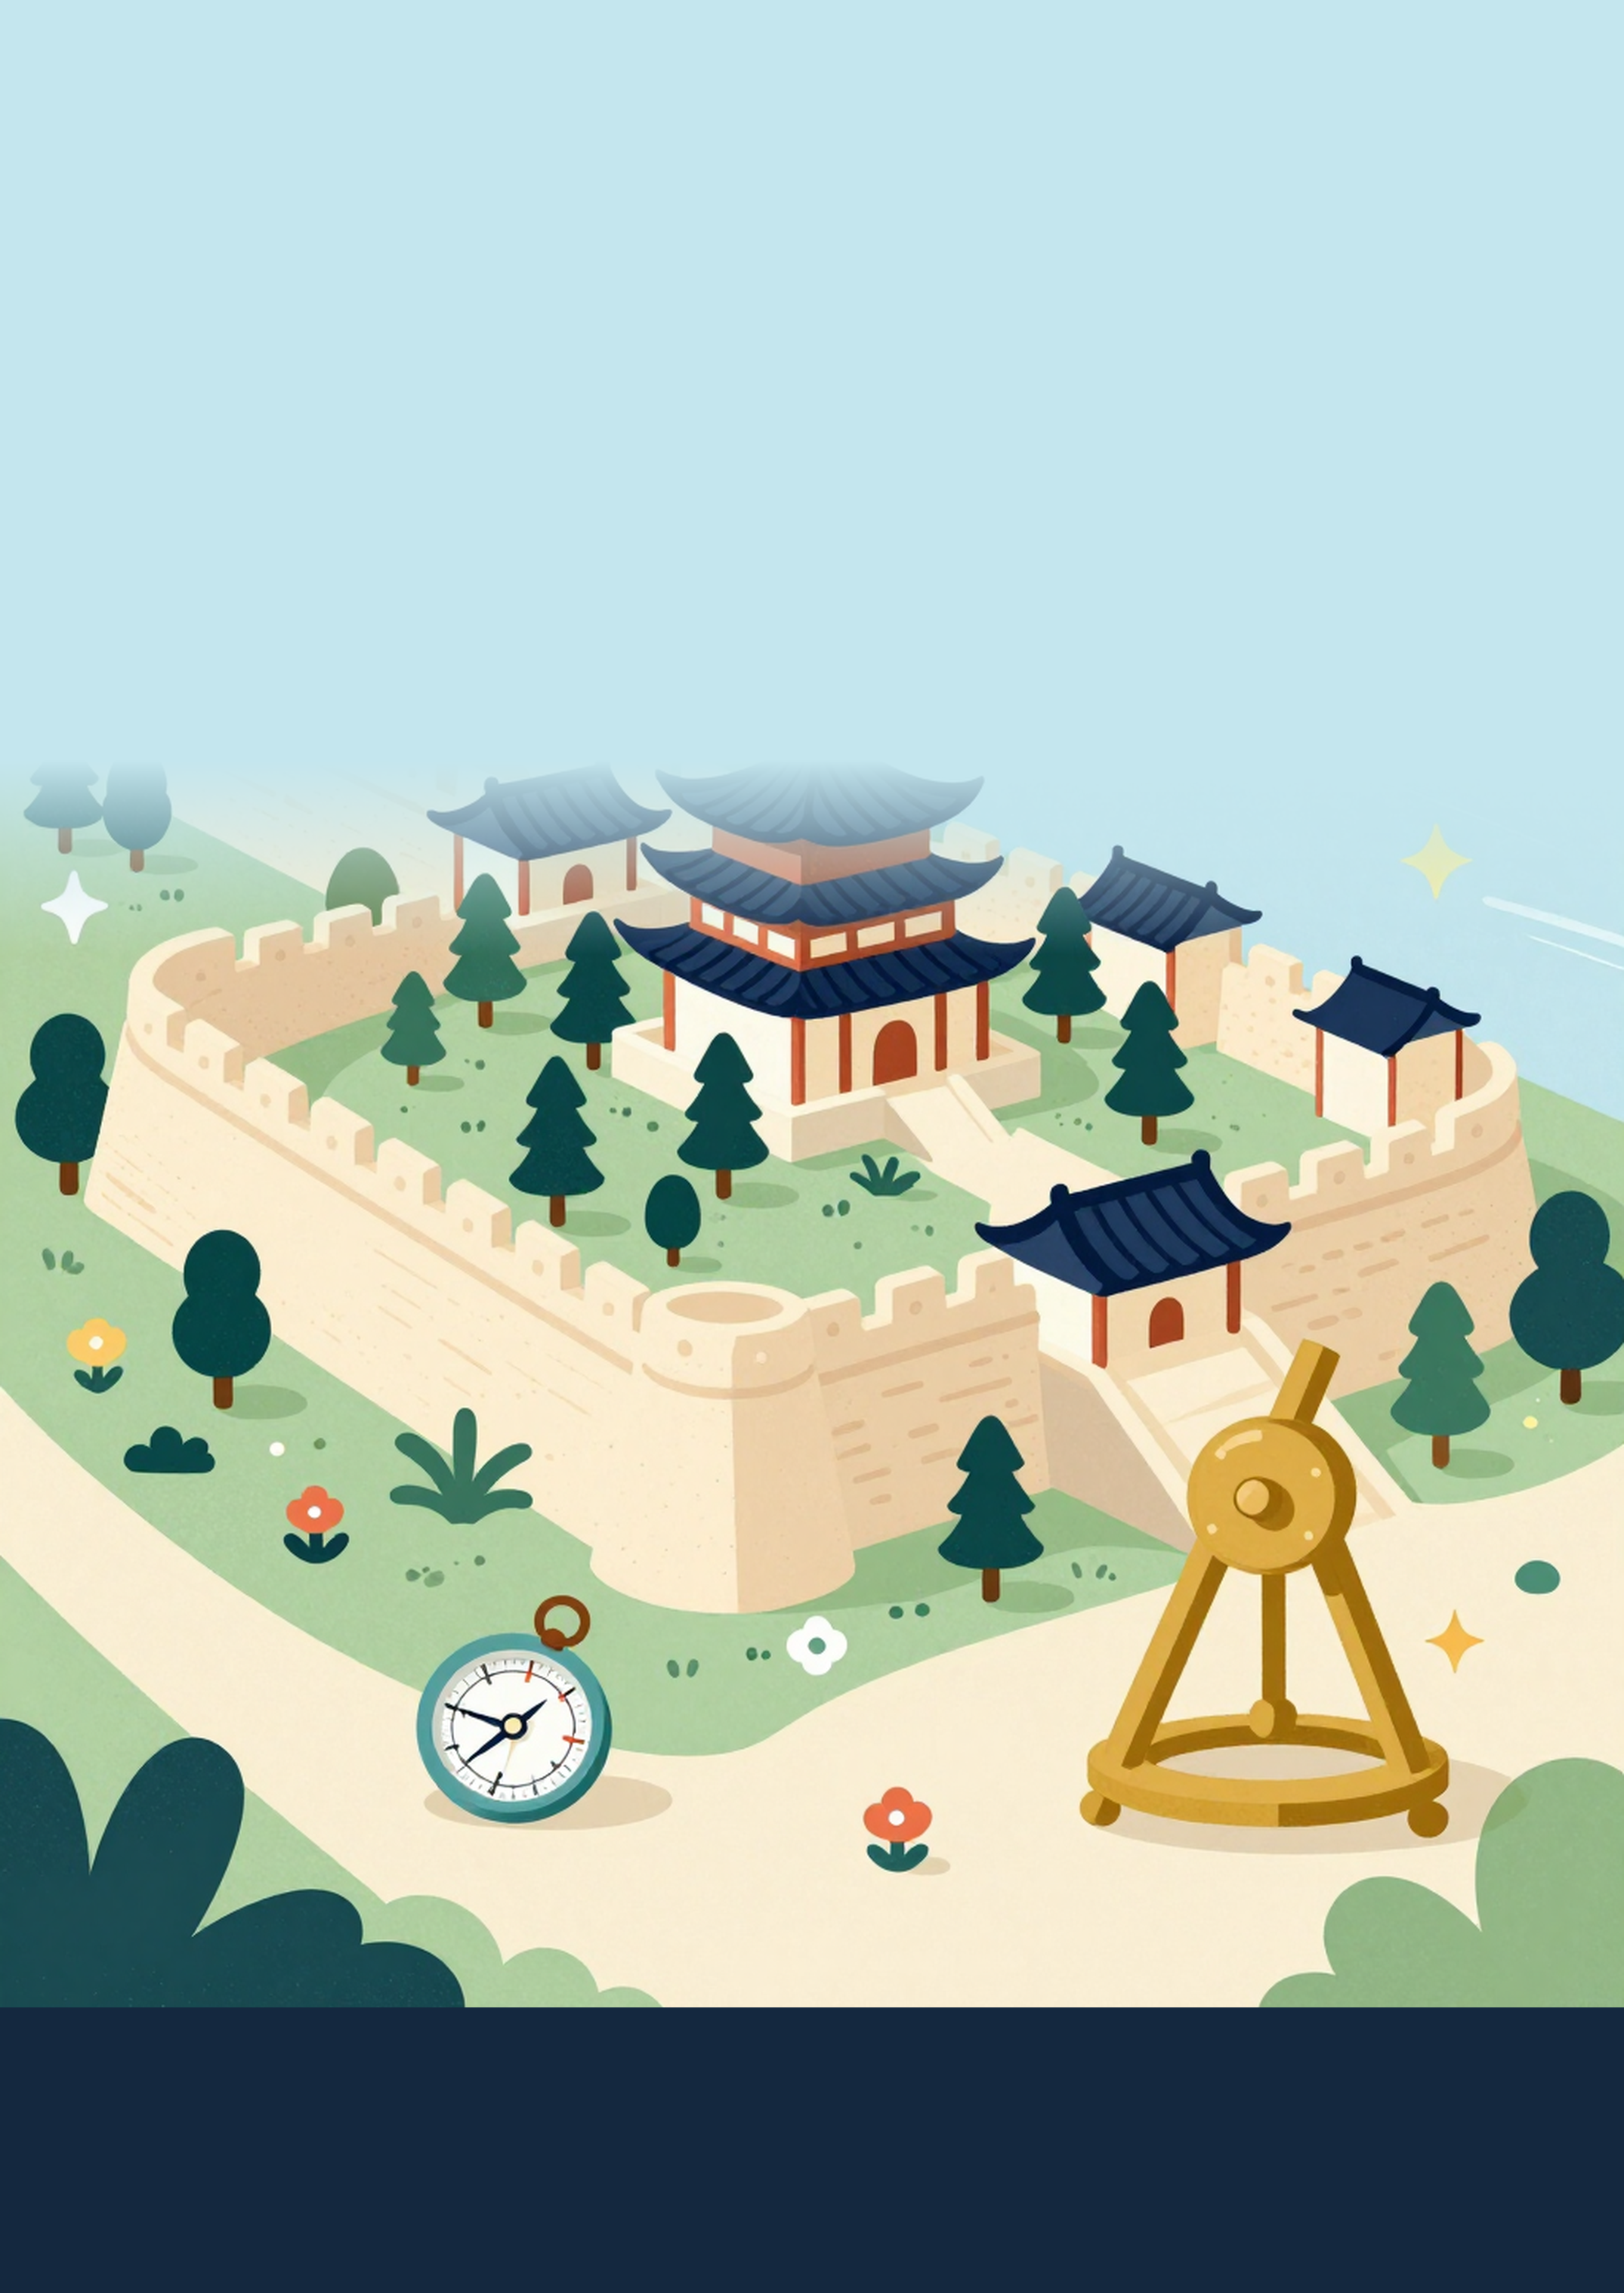
\includegraphics[width=182mm,height=257mm]{cover-v3-front.png}};
\node[anchor=north west,text=navy,align=left,font=\sffamily\bfseries\fontsize{27}{38}\selectfont] at ([xshift=16mm,yshift=-18mm]current page.north west) {고려 서경\\[-2pt](西京)의\\[-2pt]위치를\\[-2pt]추정하다};
\node[anchor=north west,text=navy!85!black,align=left,font=\sffamily\large] at ([xshift=16mm,yshift=-76mm]current page.north west) {여덟 가지 방법으로\\[2pt]동아시아 고전 지명을\\[2pt]좌표로 옮기기};
\node[anchor=south west,text=white,font=\sffamily\bfseries\Large] at ([xshift=16mm,yshift=19mm]current page.south west) {1권\quad 방법편};
\node[anchor=south west,text=white,font=\sffamily\normalsize] at ([xshift=16mm,yshift=9mm]current page.south west) {이광조 지음};
\node[anchor=south east,text=gold,font=\sffamily\normalsize] at ([xshift=-16mm,yshift=9mm]current page.south east) {과학과영성출판사};
\end{tikzpicture}
\newpage
% 뒤표지
\begin{tikzpicture}[remember picture,overlay]
\fill[paper] (current page.south west) rectangle (current page.north east);
\node[anchor=north west,inner sep=0] at (current page.north west) {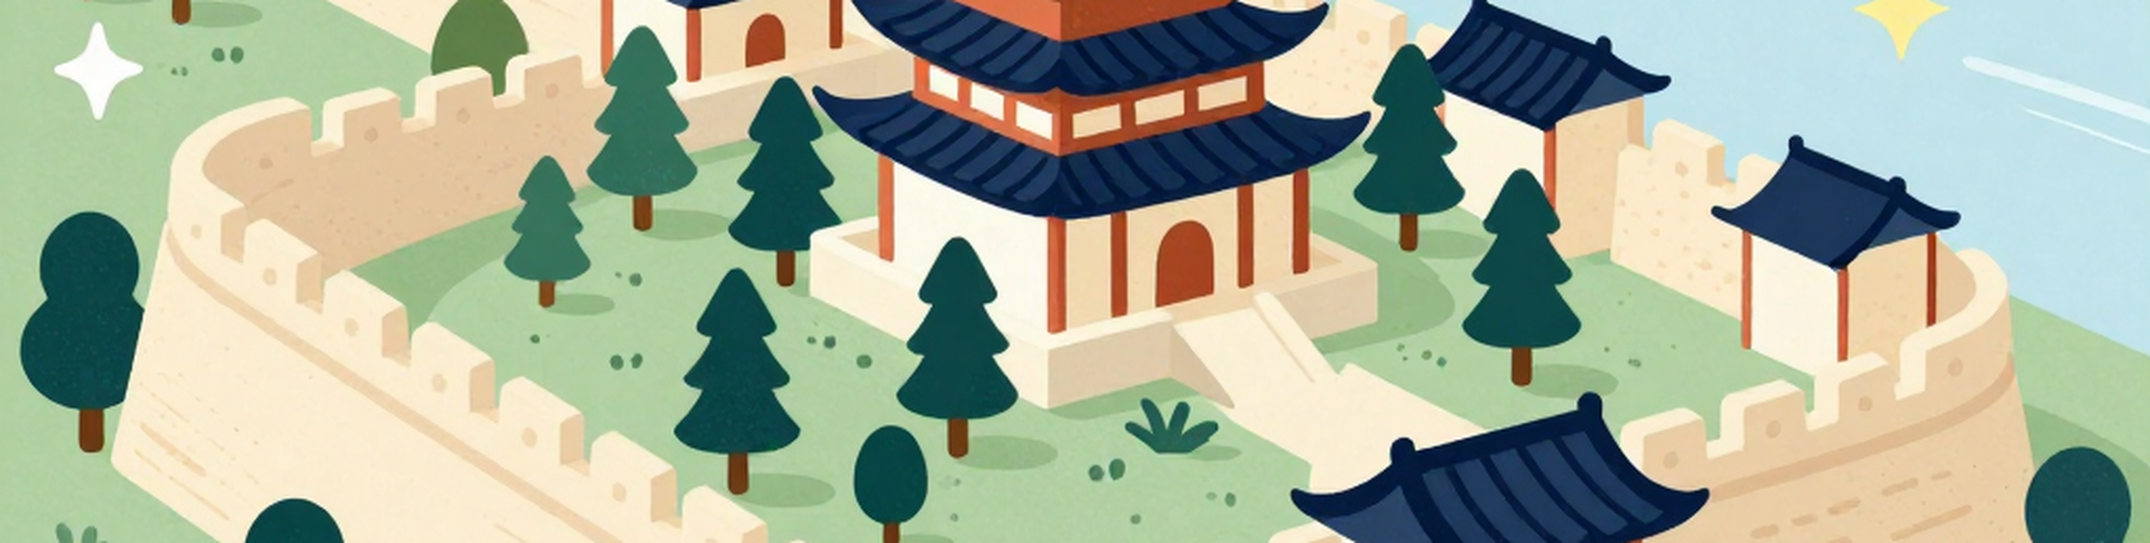
\includegraphics[width=182mm]{cover-v3-strip.png}};
\node[anchor=north west,text width=140mm,text=navy,font=\sffamily\bfseries\large] at ([xshift=18mm,yshift=-62mm]current page.north west) {옛 기록의 ``서쪽으로 십 리''를 지도 위의 점으로};
\node[anchor=north west,text width=140mm,text=black!80,font=\sffamily\normalsize,align=left] at ([xshift=18mm,yshift=-82mm]current page.north west) {%
이 책은 옛 문헌에 적힌 방위와 거리, 이웃 지명, 산과 강의 서술을 현대 지도의 좌표와 면적으로 바꾸는 여덟 가지 방법을 처음부터 차근차근 설명합니다.\par\vspace{4mm}
제약 전파, 지오레퍼런싱, 베이즈 추정, 최소비용경로 같은 기법을 중학교 2학년 수준의 말로 풀고, 실제 사료의 문장 형태를 본뜬 사례를 입력표부터 결과 해석까지 손으로 계산해 보입니다.\par\vspace{4mm}
고려 서경(西京)의 위치를 추정하는 문제를 끝까지 따라가며, 어떤 증거를 계산에 넣고 어떤 해석은 넣지 않는지를 구분하는 법을 함께 익힙니다.};
\draw[navy,line width=0.5pt,fill=white] ([xshift=-58mm,yshift=18mm]current page.south east) rectangle ([xshift=-18mm,yshift=43mm]current page.south east);
\node[text=black!50,font=\sffamily\tiny,align=center] at ([xshift=-38mm,yshift=30.5mm]current page.south east) {ISBN 바코드 자리\\(ISBN 부여 후 삽입)};
\node[anchor=south west,text=navy,font=\sffamily\small,align=left] at ([xshift=18mm,yshift=18mm]current page.south west) {과학과영성출판사\\[2pt]www.ssbook.kr\quad contact@ssbook.kr};
\end{tikzpicture}
\end{document}
